% ============================================================
%  J1 — APRÈS-MIDI : Principes du ML & Régression Linéaire
%  Julien Rolland — M2 Développement Fullstack
% ============================================================
\documentclass[aspectratio=169, 10pt]{beamer}
% ============================================================
%  PREAMBLE COMMUN — IA, Deep Learning & Machine Learning
%  Julien Rolland — M2 Développement Fullstack
% ============================================================

% --- Langue & encodage ---
\usepackage[utf8]{inputenc}
\usepackage[T1]{fontenc}
\usepackage{babel}
\babelprovide[import, main]{french}

% --- Thème Beamer ---
\usetheme{Madrid}
\usecolortheme{default}

% Palette de bleu académique
\definecolor{jedy_blue}{RGB}{0, 51, 102}       % bleu foncé principal
\definecolor{jedy_mid}{RGB}{0, 102, 179}        % bleu moyen accent
\definecolor{jedy_light}{RGB}{204, 221, 240}    % bleu très clair (fond boxes)
\definecolor{jedy_alert}{RGB}{180, 30, 30}      % rouge pour alertes
\definecolor{jedy_example}{RGB}{0, 120, 60}     % vert pour exemples

% Application des couleurs sur le thème Madrid
\setbeamercolor{palette primary}{bg=jedy_blue, fg=white}
\setbeamercolor{palette secondary}{bg=jedy_mid, fg=white}
\setbeamercolor{palette tertiary}{bg=jedy_blue, fg=white}
\setbeamercolor{palette quaternary}{bg=jedy_blue, fg=white}
\setbeamercolor{structure}{fg=jedy_blue}
\setbeamercolor{frametitle}{bg=jedy_blue, fg=white}
\setbeamercolor{title}{bg=jedy_blue, fg=white}
\setbeamercolor{block title}{bg=jedy_mid, fg=white}
\setbeamercolor{block body}{bg=jedy_light, fg=black}
\setbeamercolor{block title alerted}{bg=jedy_alert, fg=white}
\setbeamercolor{block body alerted}{bg=jedy_light, fg=black}
\setbeamercolor{block title example}{bg=jedy_example, fg=white}
\setbeamercolor{block body example}{bg=jedy_light, fg=black}

% --- Typographie ---
\usepackage{lmodern}
\setbeamerfont{title}{size=\Large, series=\bfseries}
\setbeamerfont{frametitle}{size=\normalsize, series=\bfseries}

% --- Navigation : suppression des icônes de navigation par défaut ---
\setbeamertemplate{navigation symbols}{}

% --- Numérotation des slides ---
\setbeamertemplate{footline}{%
  \leavevmode%
  \hbox{%
    \begin{beamercolorbox}[wd=.333\paperwidth,ht=2.25ex,dp=1ex,center]{author in head/foot}%
      \usebeamerfont{author in head/foot}\insertshortauthor
    \end{beamercolorbox}%
    \begin{beamercolorbox}[wd=.334\paperwidth,ht=2.25ex,dp=1ex,center]{title in head/foot}%
      \usebeamerfont{title in head/foot}\insertshorttitle
    \end{beamercolorbox}%
    \begin{beamercolorbox}[wd=.333\paperwidth,ht=2.25ex,dp=1ex,right]{date in head/foot}%
      \usebeamerfont{date in head/foot}
      \insertframenumber{} / \inserttotalframenumber\hspace*{2ex}
    \end{beamercolorbox}%
  }%
  \vskip0pt%
}

% --- Maths ---
\usepackage{amsmath, amssymb, amsthm}
\usepackage{bm}          % vecteurs en gras : \bm{w}

% --- Code source ---
\usepackage{listings}
\usepackage{xcolor}

\lstdefinestyle{pythonstyle}{
  language=Python,
  basicstyle=\ttfamily\footnotesize,
  keywordstyle=\color{jedy_blue}\bfseries,
  commentstyle=\color{gray}\itshape,
  stringstyle=\color{jedy_example},
  numberstyle=\tiny\color{gray},
  numbers=left,
  numbersep=5pt,
  frame=single,
  framerule=0.4pt,
  rulecolor=\color{jedy_light},
  backgroundcolor=\color{jedy_light!40},
  breaklines=true,
  showstringspaces=false,
  tabsize=4,
}
\lstset{style=pythonstyle}

% Alias pratique pour code inline
\newcommand{\code}[1]{\texttt{\small#1}}

% --- Graphiques ---
\usepackage{graphicx}
\usepackage{tikz}
\usetikzlibrary{arrows.meta, positioning, shapes.geometric, fit, calc}
\usepackage{pgfplots}
\pgfplotsset{compat=1.18}

% --- Tableaux ---
\usepackage{booktabs}
\usepackage{array}

% --- Icônes (optionnel, nécessite fontawesome5) ---
% \usepackage{fontawesome5}

% --- Macros ML/DL courantes ---
\newcommand{\R}{\mathbb{R}}
\newcommand{\E}{\mathbb{E}}
\newcommand{\Loss}{\mathcal{L}}
\newcommand{\dataset}{\mathcal{D}}
\newcommand{\X}{\mathbf{X}}
\newcommand{\y}{\mathbf{y}}
\newcommand{\w}{\mathbf{w}}
\newcommand{\W}{\mathbf{W}}
\newcommand{\grad}{\nabla}
\newcommand{\T}{^{\top}}         % transposée : \X\T
\newcommand{\lr}{\alpha}         % learning rate
\newcommand{\norm}[1]{\left\|#1\right\|}

% Encadré "Objectif pédagogique" en début de section
\newenvironment{objectif}{%
  \begin{alertblock}{Objectif}%
}{%
  \end{alertblock}%
}

% --- Infos du cours (remplacer dans chaque slides.tex) ---
\author[J. Rolland]{Julien Rolland}
\institute[Jedy]{Formation M2 Développement Fullstack}


\title[ML \& Régression Linéaire]{Principes du ML \& Régression Linéaire}
\subtitle{Jour 1 — Après-midi}
\date{Jour 1}

% ============================================================
\begin{document}
% ============================================================

\begin{frame}
  \titlepage
\end{frame}

\begin{frame}{Plan du module}
  \tableofcontents
\end{frame}

% ============================================================
\section{Vocabulaire du Machine Learning}
% ============================================================

\begin{frame}{Qu'est-ce que le Machine Learning ?}
  \begin{block}{Définition (Tom Mitchell, 1997)}
    Pour une \textbf{tâche} $T$, un algorithme \textbf{apprend} si sa
    \textbf{performance} $P$ sur $T$ s'améliore avec l'\textbf{expérience} $E$.
  \end{block}

  \bigskip
  \begin{columns}[T]
    \begin{column}{0.48\textwidth}
      \begin{tabular}{lll}
        \toprule
        & \textbf{Concept} & \textbf{En pratique} \\
        \midrule
        $T$ & Tâche       & Prédire un prix \\
        $P$ & Performance & Erreur MSE \\
        $E$ & Expérience  & Dataset d'entraînement \\
        \bottomrule
      \end{tabular}

      \bigskip
      \begin{exampleblock}{Paradigme clé}
        On ne \textbf{programme} plus les règles.\\
        On \textbf{montre des exemples} — le modèle induit les règles.
      \end{exampleblock}
    \end{column}
    \begin{column}{0.48\textwidth}
      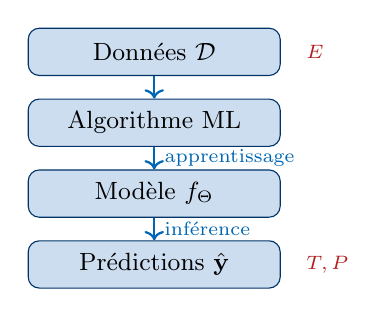
\begin{tikzpicture}[
        node distance=0.9cm,
        box/.style={draw=jedy_blue, fill=jedy_light, rounded corners,
                    minimum width=3.2cm, minimum height=0.6cm,
                    font=\small, align=center},
        arr/.style={->, jedy_mid, thick},
      ]
        \node[box] (data) {Données $\dataset$};
        \node[box, below of=data] (algo) {Algorithme ML};
        \node[box, below of=algo] (model) {Modèle $f_\Theta$};
        \node[box, below of=model] (pred) {Prédictions $\hat{\y}$};

        \draw[arr] (data)  -- (algo);
        \draw[arr] (algo)  -- node[right, font=\scriptsize]{apprentissage} (model);
        \draw[arr] (model) -- node[right, font=\scriptsize]{inférence} (pred);

        \node[right=0.2cm of data,  font=\scriptsize, jedy_alert] {$E$};
        \node[right=0.2cm of pred,  font=\scriptsize, jedy_alert] {$T, P$};
      \end{tikzpicture}
    \end{column}
  \end{columns}
\end{frame}

% ---

\begin{frame}{Les 3 Paradigmes d'Apprentissage}
  \begin{columns}[T]
    \begin{column}{0.32\textwidth}
      \begin{block}{\centering Supervisé}
        \centering
        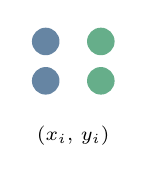
\begin{tikzpicture}
          \node[circle, fill=jedy_blue!60,    minimum size=0.35cm] at (0,    0)    {};
          \node[circle, fill=jedy_example!60, minimum size=0.35cm] at (0.7,  0)    {};
          \node[circle, fill=jedy_blue!60,    minimum size=0.35cm] at (0,   -0.5)  {};
          \node[circle, fill=jedy_example!60, minimum size=0.35cm] at (0.7, -0.5)  {};
          \node[font=\scriptsize] at (0.35, -1.2) {$(x_i,\, y_i)$};
        \end{tikzpicture}

        \vspace{0.3em}
        Données \textbf{étiquetées}\\[0.3em]
        \textit{Régression, Classification}
      \end{block}
    \end{column}
    \begin{column}{0.32\textwidth}
      \begin{block}{\centering Non-supervisé}
        \centering
        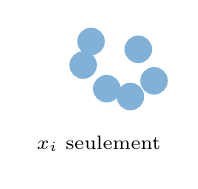
\begin{tikzpicture}
          \node[circle, fill=jedy_mid!50, minimum size=0.35cm] at (0.2,  0.1)  {};
          \node[circle, fill=jedy_mid!50, minimum size=0.35cm] at (0.9,  0.3)  {};
          \node[circle, fill=jedy_mid!50, minimum size=0.35cm] at (0.5, -0.2)  {};
          \node[circle, fill=jedy_mid!50, minimum size=0.35cm] at (1.1, -0.1)  {};
          \node[circle, fill=jedy_mid!50, minimum size=0.35cm] at (0.3,  0.4)  {};
          \node[circle, fill=jedy_mid!50, minimum size=0.35cm] at (0.8, -0.3)  {};
          \node[font=\scriptsize] at (0.4, -0.9) {$x_i$ seulement};
        \end{tikzpicture}

        \vspace{0.3em}
        Données \textbf{sans labels}\\[0.3em]
        \textit{Clustering, Embeddings}
      \end{block}
    \end{column}
    \begin{column}{0.32\textwidth}
      \begin{block}{\centering Renforcement}
        \centering
        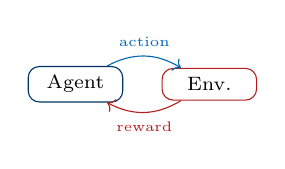
\begin{tikzpicture}[scale=0.85]
          \node[draw=jedy_blue, rounded corners, font=\scriptsize,
                minimum width=1.2cm] (agent) at (0,0) {Agent};
          \node[draw=jedy_alert, rounded corners, font=\scriptsize,
                minimum width=1.2cm] (env) at (2,0) {Env.};
          \draw[->, bend left=30, jedy_mid]  (agent) to
            node[above, font=\tiny]{action} (env);
          \draw[->, bend left=30, jedy_alert] (env) to
            node[below, font=\tiny]{reward} (agent);
        \end{tikzpicture}

        \vspace{0.3em}
        Apprentissage par \textbf{récompense}\\[0.3em]
        \textit{Jeux, Robotique}
      \end{block}
    \end{column}
  \end{columns}

  \bigskip
  \begin{alertblock}{Ce cours}
    Focus sur l'\textbf{apprentissage supervisé} (J1--J4) et les outils de mise en production (J5).
    Le non-supervisé apparaît en J4 (embeddings).
  \end{alertblock}
\end{frame}

% ---

\begin{frame}{Apprentissage Supervisé — Les Objets Mathématiques}
  \begin{columns}[T]
    \begin{column}{0.52\textwidth}
      \textbf{Dataset} $\dataset = \{(\bm{x}_i, y_i)\}_{i=1}^{N}$
      \begin{itemize}
        \item $\bm{x}_i \in \R^D$ — vecteur de \textbf{features}
        \item $y_i \in \R$ (régression) ou $\{0,1\}$ (classification)\\
              $\Rightarrow$ le \textbf{label} (ground truth)
        \item $\X \in \R^{N \times D}$ — matrice de données
      \end{itemize}

      \bigskip
      $\Theta$ = paramètres \textbf{appris} pendant l'entraînement.

      \smallskip
      \textbf{Modèle} $f_\Theta$ — appliqué à $\bm{x}_i$ donne une \textbf{prédiction} :
      \[
        \hat{y}_i = f_\Theta(\bm{x}_i)
      \]

      \bigskip
      \textbf{Apprentissage} = trouver $\Theta^*$ qui minimise\\
      l'écart entre $\hat{y}_i$ et $y_i$ :
      \[
        \Theta^* = \arg\min_\Theta\; \Loss(\hat{\y},\, \y)
      \]
    \end{column}
    \begin{column}{0.44\textwidth}
      \hspace*{-1.2cm}%
      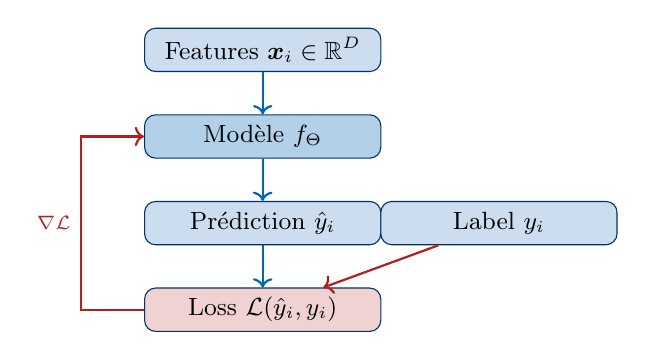
\begin{tikzpicture}[
        every node/.style={font=\small},
        box/.style={draw=jedy_blue, fill=jedy_light, rounded corners,
                    minimum width=3.0cm, minimum height=0.55cm, align=center},
      ]
        \node[box]                    (x)    at (0, 0)   {Features $\bm{x}_i \in \R^D$};
        \node[box, fill=jedy_mid!30]  (model) at (0,-1.1) {Modèle $f_\Theta$};
        \node[box]                    (yhat) at (0,-2.2) {Prédiction $\hat{y}_i$};
        \node[box, fill=jedy_alert!20](loss) at (0,-3.3) {Loss $\Loss(\hat{y}_i, y_i)$};
        \node[box]                    (gt)   at (3,-2.2) {Label $y_i$};

        \draw[->, jedy_mid, thick] (x)     -- (model);
        \draw[->, jedy_mid, thick] (model) -- (yhat);
        \draw[->, jedy_mid, thick] (yhat)  -- (loss);
        \draw[->, jedy_alert, thick] (gt)  -- (loss);
        \draw[->, jedy_alert, thick]
          (loss.west) -- ++(-0.8, 0)
          -- node[left, font=\scriptsize]{$\nabla\Loss$} ++(0, 2.2)
          -- (model.west);
      \end{tikzpicture}
    \end{column}
  \end{columns}
\end{frame}

% ============================================================
\section{Régression Linéaire}
% ============================================================

\begin{frame}{Régression — La Tâche}
  \begin{columns}[T]
    \begin{column}{0.50\textwidth}
      \textbf{Objectif :} prédire une sortie \textbf{continue} $y \in \R$
      à partir de features $\bm{x} \in \R^D$.

      \bigskip
      \textbf{Exemples :}
      \begin{itemize}
        \item Surface + localisation $\to$ prix d'un logement
        \item Historique météo $\to$ température demain
        \item Âge + poids $\to$ glycémie
      \end{itemize}

      \bigskip
      On cherche $f : \R^D \to \R$ telle que $f(\bm{x}_i) \approx y_i$.
    \end{column}
    \begin{column}{0.46\textwidth}
      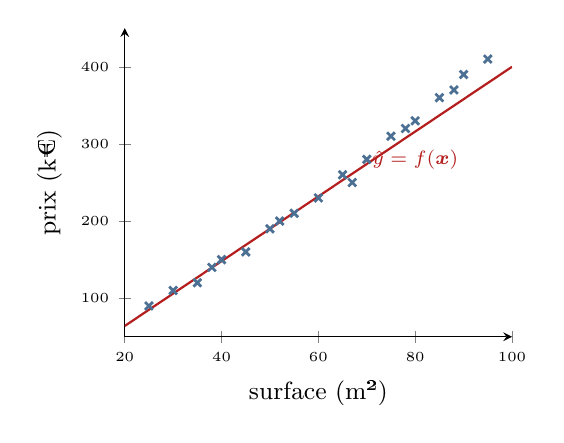
\begin{tikzpicture}
        \begin{axis}[
          width=6.5cm, height=5.5cm,
          xlabel={surface (m²)}, ylabel={prix (k€)},
          axis lines=left,
          tick label style={font=\tiny},
          label style={font=\small},
          xmin=20, xmax=100, ymin=50, ymax=450,
        ]
          \addplot[only marks, mark=x, mark size=2pt,
                   jedy_blue!70, mark options={line width=1pt}]
            coordinates {
              (25,90)(30,110)(35,120)(40,150)(45,160)
              (50,190)(55,210)(60,230)(65,260)(70,280)
              (75,310)(80,330)(85,360)(90,390)(95,410)
              (38,140)(52,200)(67,250)(78,320)(88,370)
            };
          \addplot[jedy_alert, thick, domain=20:100] {4.2*x - 20};
          \node[jedy_alert, font=\scriptsize] at (axis cs:80, 280)
            {$\hat{y} = f(\bm{x})$};
        \end{axis}
      \end{tikzpicture}
    \end{column}
  \end{columns}
\end{frame}

% ---

\begin{frame}{Régression — Choix du Modèle}
  \begin{block}{Modèle linéaire ($D=1$)}
    \[ f_{w,b}(x) = wx + b \]
  \end{block}

  \medskip
  \begin{block}{Modèle linéaire (multivarié)}
    \[ f_{\w,b}(\bm{x}) = \w\T\bm{x} + b = \sum_{j=1}^D w_j x_j + b \]
  \end{block}

  \medskip
  \begin{block}{Modèle polynomial (feature map $\Phi$)}
    \[ f_\Theta(\bm{x}) = \bm{\theta}\T \Phi(\bm{x}) \]
    \textit{Ex :} $\Phi(x) = [1, x, x^2, x^3]$ pour degré 3.
  \end{block}
\end{frame}

% ---

\begin{frame}{Fonction de Coût — La MSE}
  \begin{block}{Mean Squared Error (MSE)}
    \[
      \Loss = \frac{1}{N} \sum_{i=1}^{N} \bigl(f_\Theta(\bm{x}_i) - y_i\bigr)^2
      = \frac{1}{N} \norm{\hat{\y} - \y}^2
    \]
    \centering
    avec $\hat{\y} = [f_\Theta(\bm{x}_1), \dots, f_\Theta(\bm{x}_N)]\T \in \R^N$ le vecteur des prédictions.
  \end{block}
\end{frame}

% ---

\begin{frame}{MSE — Justification par la Vraisemblance}
  \footnotesize
  \[
    \begin{aligned}
      & \textbf{Hypothèse :}\quad y_i \sim \mathcal{N}(\hat{y}_i, \sigma^2) \text{ avec } \hat{y}_i = f_\theta(x_i) \quad\text{(bruit gaussien)} \\[0.15em]
      \implies & L = \prod_{i=1}^{n} \frac{1}{\sqrt{2\pi\sigma^2}} \exp\!\left( -\frac{(y_i - \hat{y}_i)^2}{2\sigma^2} \right) \\[0.15em]
      \implies & \ln L = \sum_{i=1}^{n} \left[ \ln\!\left(\frac{1}{\sqrt{2\pi\sigma^2}}\right) - \frac{(y_i - \hat{y}_i)^2}{2\sigma^2} \right] \\[0.15em]
      \implies & \operatorname{argmax}_{\theta} \ln L \iff \operatorname{argmax}_{\theta} \!\left( -\sum_{i=1}^{n} (y_i - \hat{y}_i)^2 \right) \\[0.15em]
      \implies & \operatorname{argmax}_{\theta} \ln L \iff \operatorname{argmin}_{\theta} \sum_{i=1}^{n} (y_i - \hat{y}_i)^2 \\[0.15em]
      \implies & \operatorname{argmin}_{\theta} \tfrac{1}{n}\sum_{i=1}^{n} (y_i - \hat{y}_i)^2 \iff \mathbf{argmin\ MSE}
    \end{aligned}
  \]
\end{frame}

% ---

\begin{frame}{Régression Linéaire — Récapitulatif du Problème}
  \begin{columns}[T]
    \begin{column}{0.50\textwidth}
      \textbf{Données} $\dataset = \{(\bm{x}_i, y_i)\}_{i=1}^{N}$
      \begin{itemize}
        \item $\bm{x}_i \in \R^D$ — features (surface, nb pièces…)
        \item $y_i \in \R$ — valeur cible à prédire (prix…)
      \end{itemize}

      \bigskip
      \textbf{Modèle} — une droite (ou hyperplan) :
      \[
        \hat{y}_i = \w\T\bm{x}_i + b
      \]
      On cherche $\w \in \R^D$ et $b \in \R$ qui \textbf{ajustent} cette droite aux données.

      \bigskip
      \textbf{Objectif} — minimiser l'erreur quadratique :
      \[
        \operatorname{argmin}_{\w,\, b}\; \frac{1}{N}\sum_{i=1}^{N}\bigl(\hat{y}_i - y_i\bigr)^2
      \]
      Trouver la droite la \textbf{plus proche} de tous les points.
    \end{column}
    \begin{column}{0.46\textwidth}
      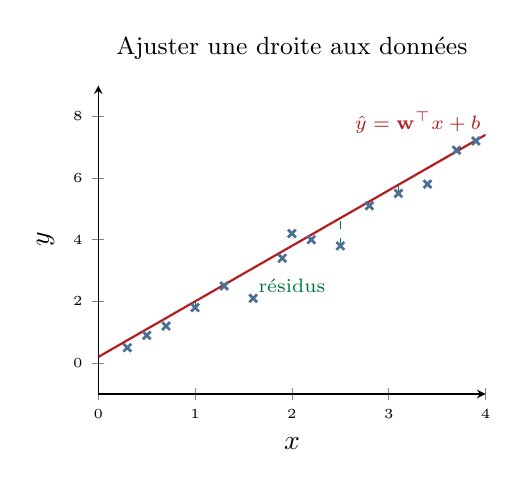
\begin{tikzpicture}
        \begin{axis}[
          width=6.5cm, height=5.5cm,
          xlabel={$x$}, ylabel={$y$},
          axis lines=left,
          tick label style={font=\tiny},
          xmin=0, xmax=4, ymin=-1, ymax=9,
          title={\small Ajuster une droite aux données},
          title style={font=\small},
        ]
          \addplot[only marks, mark=x, mark size=2pt,
                   jedy_blue!70, mark options={line width=1pt}]
            coordinates {
              (0.3,0.5)(0.7,1.2)(1.0,1.8)(1.3,2.5)(1.6,2.1)
              (1.9,3.4)(2.2,4.0)(2.5,3.8)(2.8,5.1)(3.1,5.5)
              (3.4,5.8)(3.7,6.9)(3.9,7.2)(0.5,0.9)(2.0,4.2)
            };
          \addplot[jedy_alert, thick, domain=0:4] {1.8*x + 0.2};
          % Résidus
          \draw[jedy_example, dashed, thin] (axis cs:1.0,1.8) -- (axis cs:1.0,2.0);
          \draw[jedy_example, dashed, thin] (axis cs:2.5,3.8) -- (axis cs:2.5,4.7);
          \draw[jedy_example, dashed, thin] (axis cs:3.1,5.5) -- (axis cs:3.1,5.78);
          \node[jedy_alert, font=\scriptsize] at (axis cs:3.3,7.8) {$\hat{y}=\w\T x+b$};
          \node[jedy_example, font=\scriptsize] at (axis cs:2.0,2.5) {résidus};
        \end{axis}
      \end{tikzpicture}
    \end{column}
  \end{columns}
\end{frame}

% ---

\begin{frame}[fragile]{Trick — Données Augmentées}
  \begin{columns}[T]
    \begin{column}{0.52\textwidth}
      \textbf{Problème :} gérer le biais $b$ séparément est fastidieux.
      \[
        \hat{y}_i = \w\T\bm{x}_i + b
        \quad \Rightarrow \quad
        \text{deux termes à maintenir}
      \]

      \textbf{Astuce :} ajouter une colonne de 1 dans $\X$ :
      \[
        \tilde{\bm{x}}_i =
        \begin{pmatrix} 1 \\ x_{i,1} \\ \vdots \\ x_{i,D} \end{pmatrix}
        \in \R^{D+1}
        \qquad
        \tilde{\w} =
        \begin{pmatrix} b \\ w_1 \\ \vdots \\ w_D \end{pmatrix}
      \]
      \[
        \hat{y}_i = \tilde{\w}\T \tilde{\bm{x}}_i
        \quad \Leftarrow \text{un seul terme !}
      \]
    \end{column}
    \begin{column}{0.44\textwidth}
      \textbf{En NumPy :}
\begin{lstlisting}
# X : (N, D)  ->  X_aug : (N, D+1)
ones = np.ones((N, 1))
X_aug = np.hstack([ones, X])
# w_aug contient [b, w1, ..., wD]

# Prediction
y_hat = X_aug @ w_aug
\end{lstlisting}
      \begin{exampleblock}{Avantage}
        Toutes les équations (gradient, solution analytique)
        s'écrivent \textbf{sans cas particulier} pour $b$.
      \end{exampleblock}
    \end{column}
  \end{columns}
\end{frame}

% ---

\begin{frame}{Gradient de la MSE}
  \begin{columns}[T]
    \begin{column}{0.55\textwidth}
      \begin{block}{}
        \[
          \begin{aligned}
            \Loss &= \frac{1}{N} \norm{\hat{\y} - \y}^2 \\[0.1em]
                  &= \frac{1}{N} (\X\w - \y)\T (\X\w - \y) \\[0.1em]
                  &= \frac{1}{N} \bigl(\w\T\X\T\X\w - 2\w\T\X\T\y + \y\T\y\bigr) \\[0.5em]
            \nabla_\w \Loss &= \frac{1}{N} \bigl(2\X\T\X\w - 2\X\T\y\bigr) \\[0.1em]
            \nabla_\w \Loss &= \frac{2}{N}\,\X\T (\X\w - \y)
          \end{aligned}
        \]
      \end{block}
    \end{column}
    \begin{column}{0.41\textwidth}
      \begin{alertblock}{Résultat}
        \[
          \nabla_\w \Loss = \frac{2}{N}\,\X\T (\X\w - \y)
        \]
      \end{alertblock}

      \medskip
      \begin{block}{Convexité}
        \[
          \nabla^2_\w \Loss = \frac{2}{N}\,\X\T\X
        \]
        $\X\T\X$ est une matrice de Gram :
        \[
          \forall \bm{v} \in \R^D,\quad
          \bm{v}\T(\X\T\X)\bm{v} = \norm{\X\bm{v}}^2 \geq 0
        \]
        $\Rightarrow \nabla^2_\w \Loss \succeq 0$
        $\Rightarrow$ \textbf{minimum global unique}.
      \end{block}
    \end{column}
  \end{columns}
\end{frame}

% ---

\begin{frame}{Solution analytique}
  La MSE est convexe : son minimum est atteint quand le gradient s'annule.

  \medskip
  \[
    \nabla_\w \Loss = 0
    \implies \frac{2}{N}\X\T(\X\w - \y) = 0
    \implies \X\T\X\w = \X\T\y
  \]

  \medskip
  \[
    \boxed{\w^* = (\X\T\X)^{-1}\X\T\y}
  \]

  \bigskip
  \begin{columns}[T]
    \begin{column}{0.48\textwidth}
      \begin{exampleblock}{Avantages}
        \begin{itemize}
          \item Solution \textbf{exacte} en un calcul
          \item Pas d'hyperparamètre ($\lr$, nb itérations)
        \end{itemize}
      \end{exampleblock}
    \end{column}
    \begin{column}{0.48\textwidth}
      \begin{alertblock}{Limites}
        \begin{itemize}
          \item Inverser $\X\T\X \in \R^{D\times D}$ coûte $\mathcal{O}(D^3)$
          \item Inutilisable si $D$ ou $N$ est très grand
          \item Ne généralise pas aux modèles non-linéaires
        \end{itemize}
      \end{alertblock}
    \end{column}
  \end{columns}

  \bigskip
  \begin{center}
    \small $\Rightarrow$ En pratique on préfère la \textbf{descente de gradient}, généralisable à tout modèle.
  \end{center}
\end{frame}

% ============================================================
\section{Descente de Gradient}
% ============================================================

\begin{frame}{Descente de Gradient — Intuition Géométrique}
  \begin{columns}[T]
    \begin{column}{0.50\textwidth}
      On cherche $\w^* = \arg\min_\w \Loss(\w)$.

      \bigskip
      \textbf{Idée :} le gradient $\nabla_\w\Loss$ pointe vers la
      \textbf{plus grande pente montante}.\\
      On avance dans la \textbf{direction opposée}.

      \bigskip
      \textbf{Règle de mise à jour :}
      \[
        \boxed{
          \w \leftarrow \w - \lr\, \nabla_\w \Loss(\w)
        }
      \]

      \begin{tabular}{ll}
        $\lr$ & learning rate (hyperparamètre) \\
        $\nabla_\w \Loss$ & gradient de la loss \\
      \end{tabular}

      \bigskip
      Répéter jusqu'à \textbf{convergence}.
    \end{column}
    \begin{column}{0.46\textwidth}
      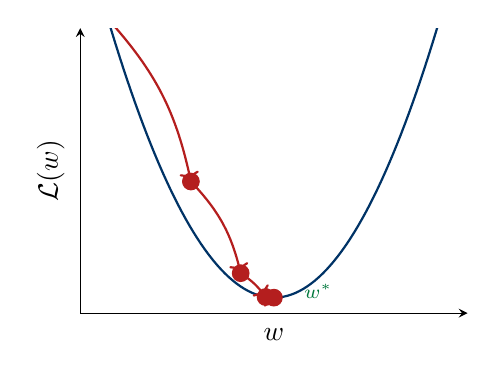
\begin{tikzpicture}
        \begin{axis}[
          width=6.5cm, height=5.2cm,
          xlabel={$w$}, ylabel={$\Loss(w)$},
          axis lines=left,
          tick label style={font=\tiny},
          xmin=-2.5, xmax=4.5, ymin=-0.2, ymax=9,
          xtick=\empty, ytick=\empty,
        ]
          % Courbe de loss
          \addplot[jedy_blue, thick, domain=-2.5:4.5, samples=100]
            {(x-1)^2 + 0.3};

          % Points de descente
          \addplot[only marks, mark=*, mark size=3pt, jedy_alert]
            coordinates {(-2, 9.3)(-0.5, 4.05)(0.4, 1.09)(0.85, 0.32)(1.0, 0.3)};

          % Fleches
          \draw[->, jedy_alert, thick] (axis cs:-2,9.3)
            to[bend left=15] (axis cs:-0.5,4.05);
          \draw[->, jedy_alert, thick] (axis cs:-0.5,4.05)
            to[bend left=15] (axis cs:0.4,1.09);
          \draw[->, jedy_alert, thick] (axis cs:0.4,1.09)
            to[bend left=10] (axis cs:0.85,0.32);
          \draw[->, jedy_alert, thick] (axis cs:0.85,0.32)
            to (axis cs:1.0,0.3);

          % Minimum
          \node[jedy_example, font=\scriptsize] at (axis cs:1.8, 0.5)
            {$w^*$};

          % Init
          \node[font=\scriptsize] at (axis cs:-2, 9.8) {init};
        \end{axis}
      \end{tikzpicture}
    \end{column}
  \end{columns}
\end{frame}

% ---

\begin{frame}[fragile]{L'Algorithme — Descente de Gradient (Batch)}
  \begin{columns}[T]
    \begin{column}{0.50\textwidth}
\begin{lstlisting}
def gradient_descent(X, y, lr, n_iters):
    N, D = X.shape
    w = np.zeros(D)        # init

    for t in range(n_iters):
        y_hat = X @ w
        error = y_hat - y  # (N,)

        grad = (2/N) * X.T @ error  # (D,)
        w = w - lr * grad

    return w
\end{lstlisting}

      \begin{alertblock}{Complexité}
        $\mathcal{O}(N \cdot D)$ par itération.\\
        Sur grand dataset : utiliser \textbf{Mini-Batch GD}.
      \end{alertblock}
    \end{column}
    \begin{column}{0.46\textwidth}
      \textbf{Variantes :}

      \medskip
      \begin{tabular}{lp{3.2cm}}
        \toprule
        Batch GD & Gradient sur \textbf{tout} le dataset \\[0.3em]
        SGD      & Gradient sur \textbf{1 exemple} aléatoire \\[0.3em]
        Mini-Batch & Gradient sur un \textbf{batch} de taille $B$ \\
        \bottomrule
      \end{tabular}

      \bigskip
      \begin{exampleblock}{En pratique}
        Mini-Batch ($B = 32$ à $256$) est le standard.\\
        C'est ce qu'utilise PyTorch avec \code{DataLoader}.
      \end{exampleblock}
    \end{column}
  \end{columns}
\end{frame}

% ---

\begin{frame}{Choix du Learning Rate $\lr$}
  \begin{columns}[T]
    \begin{column}{0.33\textwidth}
      \centering
      \textbf{$\lr$ trop petit}
      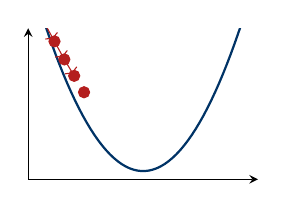
\begin{tikzpicture}
        \begin{axis}[
          width=4.5cm, height=3.5cm,
          axis lines=left, xtick=\empty, ytick=\empty,
          xmin=-2.5, xmax=4.5, ymin=-0.2, ymax=9,
        ]
          \addplot[jedy_blue, thick, domain=-2.5:4.5, samples=60]
            {(x-1)^2 + 0.3};
          \addplot[only marks, mark=*, mark size=2pt, jedy_alert]
            coordinates {(-2,9.3)(-1.7,8.2)(-1.4,7.1)(-1.1,6.1)(-0.8,5.1)};
          \draw[->, jedy_alert] (axis cs:-2,9.3) -- (axis cs:-1.7,8.2);
          \draw[->, jedy_alert] (axis cs:-1.7,8.2) -- (axis cs:-1.4,7.1);
          \draw[->, jedy_alert] (axis cs:-1.4,7.1) -- (axis cs:-1.1,6.1);
        \end{axis}
      \end{tikzpicture}
      {\small Convergence \textbf{lente}.\\Beaucoup d'itérations.}
    \end{column}
    \begin{column}{0.33\textwidth}
      \centering
      \textbf{$\lr$ adapté}
      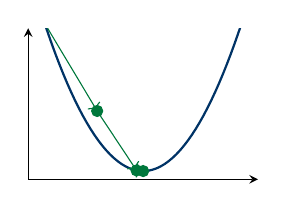
\begin{tikzpicture}
        \begin{axis}[
          width=4.5cm, height=3.5cm,
          axis lines=left, xtick=\empty, ytick=\empty,
          xmin=-2.5, xmax=4.5, ymin=-0.2, ymax=9,
        ]
          \addplot[jedy_blue, thick, domain=-2.5:4.5, samples=60]
            {(x-1)^2 + 0.3};
          \addplot[only marks, mark=*, mark size=2pt, jedy_example]
            coordinates {(-2,9.3)(-0.4,3.96)(0.8,0.34)(1.0,0.3)};
          \draw[->, jedy_example] (axis cs:-2,9.3)  -- (axis cs:-0.4,3.96);
          \draw[->, jedy_example] (axis cs:-0.4,3.96)-- (axis cs:0.8,0.34);
          \draw[->, jedy_example] (axis cs:0.8,0.34) -- (axis cs:1.0,0.3);
        \end{axis}
      \end{tikzpicture}
      {\small Convergence \textbf{rapide}.\\Atteint le minimum.}
    \end{column}
    \begin{column}{0.33\textwidth}
      \centering
      \textbf{$\lr$ trop grand}
      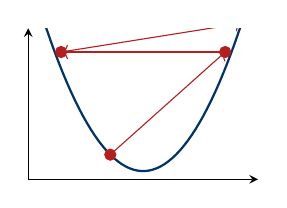
\begin{tikzpicture}
        \begin{axis}[
          width=4.5cm, height=3.5cm,
          axis lines=left, xtick=\empty, ytick=\empty,
          xmin=-2.5, xmax=4.5, ymin=-0.2, ymax=9,
        ]
          \addplot[jedy_blue, thick, domain=-2.5:4.5, samples=60]
            {(x-1)^2 + 0.3};
          \addplot[only marks, mark=*, mark size=2pt, jedy_alert]
            coordinates {(0,1.3)(3.5,7.55)(-1.5,7.55)(4,9.3)};
          \draw[->, jedy_alert] (axis cs:0,1.3)   -- (axis cs:3.5,7.55);
          \draw[->, jedy_alert] (axis cs:3.5,7.55) -- (axis cs:-1.5,7.55);
          \draw[->, jedy_alert] (axis cs:-1.5,7.55)-- (axis cs:4,9.3);
        \end{axis}
      \end{tikzpicture}
      {\small \textbf{Diverge}.\\Oscille ou explose.}
    \end{column}
  \end{columns}

  \bigskip
  \begin{block}{Règle pratique}
    Commencer à $\lr = 10^{-3}$, observer la courbe de loss.\\
    Si la loss \textbf{oscille} $\to$ diviser par 10. \quad
    Si elle \textbf{stagne} $\to$ multiplier par 3.
  \end{block}
\end{frame}

% ---

\begin{frame}{Limitations de la Descente de Gradient}
  \begin{columns}[T]
    \begin{column}{0.52\textwidth}
      \begin{alertblock}{Problèmes généraux}
        \begin{itemize}
          \item Converge vers un \textbf{minimum local}\\
                (pas nécessairement global)
          \item Résultat dépend de \textbf{l'initialisation}
          \item Peut \textbf{ne pas converger} si $\lr$ trop grand
          \item Lent sur de très grands datasets (Batch GD)
        \end{itemize}
      \end{alertblock}
    \end{column}
    \begin{column}{0.44\textwidth}
      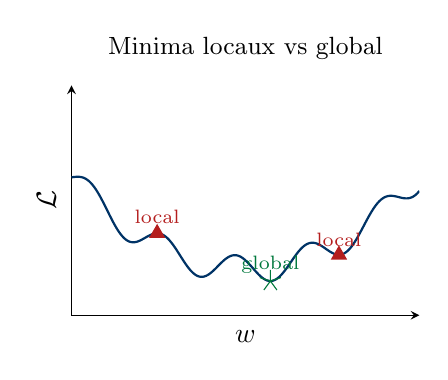
\begin{tikzpicture}
        \begin{axis}[
          width=6cm, height=4.5cm,
          xlabel={$w$}, ylabel={$\Loss$},
          axis lines=left, xtick=\empty, ytick=\empty,
          xmin=0, xmax=10, ymin=0, ymax=5,
          title={\small Minima locaux vs global},
          title style={font=\small},
        ]
          \addplot[jedy_blue, thick, domain=0:10, samples=200]
            {0.3*sin(deg(3*x)) + 0.08*(x-5)^2 + 1};
          % local min
          \addplot[only marks, mark=triangle*, mark size=3pt, jedy_alert]
            coordinates {(2.462, 1.783)(7.688, 1.314)};
          % global min
          \addplot[only marks, mark=star, mark size=4pt, jedy_example]
            coordinates {(5.717, 0.744)};
          \node[font=\scriptsize, jedy_alert]   at (axis cs:2.462, 2.15) {local};
          \node[font=\scriptsize, jedy_alert]   at (axis cs:7.688, 1.65) {local};
          \node[font=\scriptsize, jedy_example] at (axis cs:5.717, 1.10) {global};
        \end{axis}
      \end{tikzpicture}
    \end{column}
  \end{columns}

  \bigskip
  \begin{exampleblock}{Bonne nouvelle pour la régression linéaire}
    La MSE est \textbf{convexe} $\Rightarrow$ un seul minimum, GD le trouve toujours.\\
    C'est une propriété exceptionnelle — les réseaux profonds ne l'ont pas.
  \end{exampleblock}
\end{frame}

% ============================================================
% RÉCAPITULATIF
% ============================================================

\begin{frame}{Récapitulatif — Ce qu'on a vu}
  \begin{columns}[T]
    \begin{column}{0.48\textwidth}
      \begin{block}{Vocabulaire ML}
        \begin{itemize}
          \item Task $T$, Performance $P$, Experience $E$
          \item Supervisé / Non-supervisé / Renforcement
          \item Features $\X$, labels $\y$, modèle $f_\Theta$, loss $\Loss$
        \end{itemize}
      \end{block}

      \bigskip
      \begin{block}{Régression Linéaire}
        \begin{itemize}
          \item $\hat{y} = \w\T\bm{x} + b$
          \item MSE : $\Loss = \frac{1}{N}\norm{\X\w - \y}^2$
          \item Gradient : $\frac{2}{N}\X\T(\X\w - \y)$
          \item Augmented data : biais intégré dans $\w$
        \end{itemize}
      \end{block}
    \end{column}
    \begin{column}{0.48\textwidth}
      \begin{block}{Descente de Gradient}
        \begin{itemize}
          \item $\w \leftarrow \w - \lr\,\nabla_\w\Loss$
          \item Batch / SGD / Mini-Batch
          \item $\lr$ trop petit : lent \quad $\lr$ trop grand : diverge
          \item MSE convexe $\Rightarrow$ minimum global garanti
        \end{itemize}
      \end{block}
    \end{column}
  \end{columns}
\end{frame}

% ============================================================
\end{document}
